\documentclass{beamer}
\usepackage{amsmath}
\usepackage[english]{babel} %set language; note: after changing this, you need to delete all auxiliary files to recompile
\usepackage[utf8]{inputenc} %define file encoding; latin1 is the other often used option
\usepackage{csquotes} % provides context sensitive quotation facilities
\usepackage{graphicx} %allows for inserting figures
\usepackage{booktabs} % for table formatting without vertical lines
\usepackage{textcomp} % allow for example using the Euro sign with \texteuro
\usepackage{stackengine}
\usepackage{wasysym}
\usepackage{tikzsymbols}
\usepackage{textcomp}
\newcommand{\bubblethis}[2]{
        \tikz[remember picture,baseline]{\node[anchor=base,inner sep=0,outer sep=0]%
        (#1) {\underline{#1}};\node[overlay,cloud callout,callout relative pointer={(0.2cm,-0.7cm)},%
        aspect=2.5,fill=yellow!90] at ($(#1.north)+(-0.5cm,1.6cm)$) {#2};}%
    }%
\tikzset{face/.style={shape=circle,minimum size=4ex,shading=radial,outer sep=0pt,
        inner color=white!50!yellow,outer color= yellow!70!orange}}
%% Some commands to make the code easier
\newcommand{\emoticon}[1][]{%
  \node[face,#1] (emoticon) {};
  %% The eyes are fixed.
  \draw[fill=white] (-1ex,0ex) ..controls (-0.5ex,0.2ex)and(0.5ex,0.2ex)..
        (1ex,0.0ex) ..controls ( 1.5ex,1.5ex)and( 0.2ex,1.7ex)..
        (0ex,0.4ex) ..controls (-0.2ex,1.7ex)and(-1.5ex,1.5ex)..
        (-1ex,0ex)--cycle;}
\newcommand{\pupils}{
  %% standard pupils
  \fill[shift={(0.5ex,0.5ex)},rotate=80] 
       (0,0) ellipse (0.3ex and 0.15ex);
  \fill[shift={(-0.5ex,0.5ex)},rotate=100] 
       (0,0) ellipse (0.3ex and 0.15ex);}

\newcommand{\emoticonname}[1]{
  \node[below=1ex of emoticon,font=\footnotesize,
        minimum width=4cm]{#1};}
\usepackage{scalerel}
\usetikzlibrary{positioning}
\usepackage{xcolor,amssymb}
\newcommand\dangersignb[1][2ex]{%
  \scaleto{\stackengine{0.3pt}{\scalebox{1.1}[.9]{%
  \color{red}$\blacktriangle$}}{\tiny\bfseries !}{O}{c}{F}{F}{L}}{#1}%
}
\newcommand\dangersignw[1][2ex]{%
  \scaleto{\stackengine{0.3pt}{\scalebox{1.1}[.9]{%
  \color{red}$\blacktriangle$}}{\color{white}\tiny\bfseries !}{O}{c}{F}{F}{L}}{#1}%
}
\usepackage{fontawesome} % Social Icons
\usepackage{epstopdf} % allow embedding eps-figures
\usepackage{tikz} % allows drawing figures
\usepackage{amsmath,amssymb,amsthm} %advanced math facilities
\usepackage{lmodern} %uses font that support italic and bold at the same time
\usepackage{hyperref}
\usepackage{tikz}
\hypersetup{
    colorlinks=true,
    linkcolor=blue,
    filecolor=magenta,      
    urlcolor=blue,
}
\usepackage{tcolorbox}
%add citation management using BibLaTeX
\usepackage[citestyle=authoryear-comp, %define style for citations
    bibstyle=authoryear-comp, %define style for bibliography
    maxbibnames=10, %maximum number of authors displayed in bibliography
    minbibnames=1, %minimum number of authors displayed in bibliography
    maxcitenames=3, %maximum number of authors displayed in citations before using et al.
    minnames=1, %maximum number of authors displayed in citations before using et al.
    datezeros=false, % do not print dates with leading zeros
    date=long, %use long formats for dates
    isbn=false,% show no ISBNs in bibliography (applies only if not a mandatory field)
    url=false,% show no urls in bibliography (applies only if not a mandatory field)
    doi=false, % show no dois in bibliography (applies only if not a mandatory field)
    eprint=false, %show no eprint-field in bibliography (applies only if not a mandatory field)
    backend=biber %use biber as the backend; backend=bibtex is less powerful, but easier to install
    ]{biblatex}
\addbibresource{../mybibfile.bib} %define bib-file located one folder higher


\usefonttheme[onlymath]{serif} %set math font to serif ones

\definecolor{beamerblue}{rgb}{0.2,0.2,0.7} %define beamerblue color for later use

%%% defines highlight command to set text blue
\newcommand{\highlight}[1]{{\color{blue}{#1}}}


%%%%%%% commands defining backup slides so that frame numbering is correct

\newcommand{\backupbegin}{
   \newcounter{framenumberappendix}
   \setcounter{framenumberappendix}{\value{framenumber}}
}
\newcommand{\backupend}{
   \addtocounter{framenumberappendix}{-\value{framenumber}}
   \addtocounter{framenumber}{\value{framenumberappendix}}
}

%%%% end of defining backup slides

%Specify figure caption, see also http://tex.stackexchange.com/questions/155738/caption-package-not-working-with-beamer
\setbeamertemplate{caption}{\insertcaption} %redefines caption to remove label "Figure".
%\setbeamerfont{caption}{size=\scriptsize,shape=\itshape,series=\bfseries} %sets figure  caption bold and italic and makes it smaller


\usetheme{Boadilla}

%set options of hyperref package
\hypersetup{
    bookmarksnumbered=true, %put section numbers in bookmarks
    naturalnames=true, %use LATEX-computed names for links
    citebordercolor={1 1 1}, %color of border around cites, here: white, i.e. invisible
    linkbordercolor={1 1 1}, %color of border around links, here: white, i.e. invisible
    colorlinks=true, %color links
    anchorcolor=black, %set color of anchors
    linkcolor=beamerblue, %set link color to beamer blue
    citecolor=blue, %set cite color to beamer blue
    pdfpagemode=UseThumbs, %set default mode of PDF display
    breaklinks=true, %break long links
    pdfstartpage=1 %start at first page
    }


% --------------------
% Overall information
% --------------------
\title[Economía I]{Economía I \vspace{4mm}
\\ Magistral 16: Distorsiones de mercado II}
\date{}
\author[Ertola Navajas y Fariña]{Ertola Navajas y Fariña}
\vspace{0.4cm}
\institute[]{Universidad de San Andrés} 

\begin{document}

\begin{frame}
\titlepage
\centering

\includegraphics[scale=0.2]{Slides Principios de Economia/Figures/logoUDESA.jpg} 
\end{frame}


\begin{frame}{Distorsiones al equilibrio de mercado}
    \begin{itemize}
        \item Por las características de la realidad \vspace{1mm}
        \begin{itemize}
            \item Monopolios naturales (red eléctrica, agua, gas)   
             \vspace{1mm}
            \item Externalidades
             \vspace{1mm}
            \item Bienes públicos
            \vspace{1mm}
            \item Problemas de información
            \begin{itemize}
                \item Atributos ocultos (selección adversa)
                 \vspace{1mm}
                \item Acciones ocultas (moral hazard)
            \end{itemize}        
        \end{itemize}
    \end{itemize}
\end{frame}

\begin{frame}{Externalidades}
    \begin{itemize}
        \item Sucede cuando una decisión económica genera un beneficio o costo no pecuniario
        \item Afecta a terceros que no son capaces de internalizar estos beneficios o costos
        \item La clave es que estos beneficios o costos ¡no se reflejan en los precios!
        \vspace{1mm}
        \item Dos tipos de externalidades: 
        \begin{itemize}
            \item Externalidades negativas
            \vspace{1mm}
            \item Externalidades positivas
        \end{itemize}
        
    \end{itemize}
\end{frame}

\begin{frame}{Un ejemplo}
    \centering  
    \href{https://econ.video/2022/06/20/the-g-word-with-adam-conover-externalities-regulation/}{
\includegraphics[scale=0.35]{Slides Principios de Economia/Figures/ExternalidadP.png}}  
\end{frame}

\begin{frame}{Externalidades}
    \begin{itemize}
        \item ¿Que pasa con la cantidad?
        \item ¿Cual es la perdida o ganancia de la empresa?
        \item ¿Y la perdida o ganancia social?
    \end{itemize}
\end{frame}


\begin{frame}{Como se suman los costos}
    \begin{figure} [H]
\centering
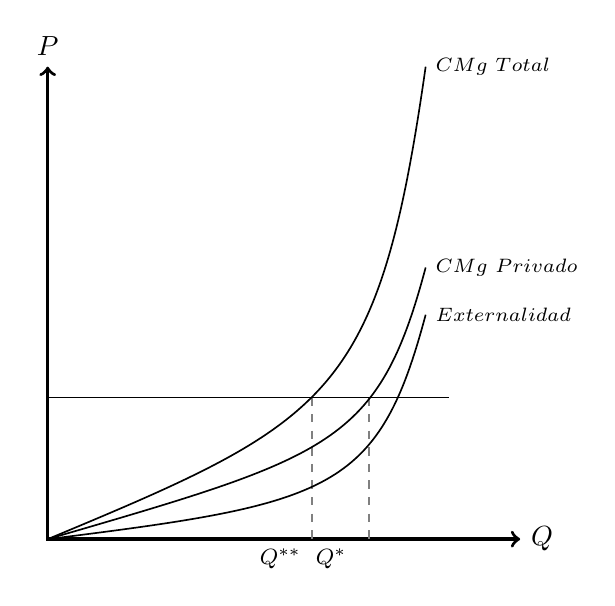
\begin{tikzpicture}[scale=0.6]
\draw[very thick,<->] (0,10) node[above]{$P$}--(0,0)--(10,0) node[right]{$Q$};
\draw[thick, dashed, gray] (5.6,3)--(5.6,0);
\draw[thick, dashed, gray] (6.8,3)--(6.8,0);
\draw [semithick] (0,0)..controls (6,1.75) and (7,2) .. (8,5.75) node [right] {\scriptsize $CMg \hspace{0.1cm} Privado$};
\draw [semithick] (0 ,0)..controls (6,0.75) and (7,1) .. (8,4.75) node [right] {\scriptsize $Externalidad$};
\draw [semithick] (0,0)..controls (6,2.5) and (7,3) .. (8,10) node [right] {\scriptsize $CMg \hspace{0.1cm} Total$};
\draw[semithick] (0,3)--(8.5,3);
\node[below] at (6,0) {\footnotesize $Q^{*}$};
\node[below] at (4.925,0) {\footnotesize $Q^{**}$};
\end{tikzpicture}
\end{figure} 
\end{frame}


 
\begin{frame}{Como corregir una externalidad....}

\end{frame}

\begin{frame}{Como corregir una externalidad}
    \begin{itemize}
        \item ¿Prohibir?
        \vspace{1mm}
        \item ¿Regular la producción o el uso del contaminante?
        \vspace{1mm}
        \item ¿Gravar (con un impuesto) la actividad contaminante?
        \item ¿Negociación privada?
    \end{itemize}
\end{frame}

\begin{frame}{Veamos...}

\end{frame}

\begin{frame}{Otro ejemplo}
    \centering  
    \href{https://econ.video/2022/06/21/the-g-word-with-adam-conover-external-benefits-of-gps/}{
\includegraphics[scale=0.35]{Slides Principios de Economia/Figures/ExternalidadPII.png}}  
\end{frame}


\begin{frame}{Externalidad positiva}
  
\end{frame}
  
\begin{frame}{Teorema de Coase}
    \begin{itemize}
        \item Coase dice que las externalidades no son un problema
        \item .... si los derechos de propiedad están bien definidos y los costos de transacción son nulos
        \item Esto es así porque ``hay una ganancia para apropiar'' de buscar un óptimo 
    \end{itemize}
\end{frame}

\begin{frame}{Coase I}
    \begin{figure} [H]
\centering
\begin{tikzpicture}[scale=0.6]
\draw[thick,<->] (0,10) node[above]{$P$}--(0,0)--(10,0) node[right]{$Q$};
\draw[fill,blue!15] (6.1,3.3)--(6.1,5)--(7.45,7.4)--(7.45,5)--(6.8,4);
%\draw[lines] (6.1,3.3)--(6.1,5)--(7.45,5)--(6.8,4);
%\draw[pattern=north west lines, pattern color=gray,solid] (6.1,3.3)--(6.1,5)--(7.45,5);
\path[pattern=horizontal lines,pattern color=black] (6.1,3.3)--(6.1,5)--(7.45,5);
\draw[thick, gray,dashed] (7.45,0)--(7.45,7.5);
\draw[thick, gray,dashed] (6.1,0)--(6.1,5);
\draw [semithick] (0,5) to (9,5) ;
\draw[semithick] (1,2)..controls (3,2) and (6,3) .. (8,9);
\draw[semithick] (1,1)..controls (3,1) and (7,2) .. (9,8.5);
\node[left] at (0,5) {\footnotesize $P^{*}$};
\node[below] at (7.45,0) {\footnotesize $Q^{*}$};
\node[below] at (6.1,0) {\footnotesize $Q^{**}$};
 \draw[semithick, <-] (6.75,4).. controls (7.15,3.75) and (7.7,3.75) ..(8.5,4);
\node [right] at (8.9,4.15) {\scriptsize Pérdida potencial};
\node [right] at (8.5,3.75) {\scriptsize Curtiembres};
\draw[semithick, <-] (6.85,5.8)--(5.75,7);
\node [right] at (3.75,7.75) {\scriptsize Pérdida Total};
\node [right] at (4.1,7.35) {\scriptsize Pescadores};

\end{tikzpicture}
\end{figure} 
\end{frame}
 
\begin{frame}{Coase II}
    \begin{figure} [H]
\centering
\begin{tikzpicture}[scale=0.6]
\draw[thick,<->] (0,10) node[above]{$P$}--(0,0)--(10,0) node[right]{$Q$};
\draw[fill,blue!15] (0.05,1.05)--(0.05,3)--(4.05,3)--(4.05,1.8)--(2,1.14)--(1,1.05);
\path[pattern=vertical lines,pattern color=black] (0,1)--(0,2)--(1.5,2)--(3,2.4)--(4.05,3)--(4.05,1.8)--(3,1.45)--(1.5,1.1);
\draw[thick, gray,dashed] (4.05,0)--(4.05,3);
\draw [semithick] (0,3) to (9,3) ;
\draw[semithick] (0.25,2)..controls (3,2) and (6,3) .. (8,9);
\draw[semithick] (0.25,1)..controls (3,1) and (7,2) .. (9,8.5);
\node[left] at (0,3) {\footnotesize $P^{*}$};
\node[below] at (4.05,0) {\footnotesize $Q^{**}$};
\draw[semithick, ->] (-0.5,1.5)--(0.5,1.5);
\draw[semithick, <-] (1.5,2.65)--(1.5,3.75);   
\node [right] at (0.5,4.5) {\scriptsize Ganancia };
   \node [right] at (0.25,4.1) {\scriptsize Curtiembres};
         \node [right] at (-3,1.75) {\scriptsize Pérdida };
   \node [right] at (-3.25,1.35) {\scriptsize Pescadores};
\end{tikzpicture}
\end{figure} 
\end{frame}

\begin{frame}{Bienes Públicos}
\begin{itemize}
    \item Vamos a distinguir los bienes por dos características
    \begin{itemize}
        \item Si su consumo es rival
        \item Si su consumo es excluible
    \end{itemize}
\end{itemize}
\end{frame}

\begin{frame}{Bienes Públicos}
\begin{table}[]
    \centering
    \begin{tabular}{|c|c|c|}
\hline
                      & \textbf{Rival}   & \textbf{No rival} \\ \hline
\textbf{Excluible}    & Bienes privados  & Bienes club       \\ \hline
\textbf{No Excluible} & Recursos comunes & Bienes públicos   \\ \hline
\end{tabular}
\end{table}
\end{frame}


\begin{frame}
\frametitle{Free rider o Homero.....}
    \centering  
    \href{https://econ.video/2017/10/26/the-simpsons-pay-what-you-want/}{
\includegraphics[scale=0.35]{Slides Principios de Economia/Figures/BienespublicosHomero.png}}  
\end{frame}


\begin{frame}
\frametitle{Ejemplo}
A los ciudadanos de Smalltown, Estados Unidos, les gusta ver los fuegos artificiales el 4 de julio, día de la independencia. \\
\vspace{3mm}
Cada uno de los 500 habitantes del pueblo atribuye un valor de \$10 a la experiencia, para un beneficio total igual a \$5000.\\
\vspace{3mm} 
El costo de montar el espectáculo de fuegos pirotécnicos es de \$1000. 
\end{frame}

\begin{frame}
\frametitle{Ejemplo}
En vista de que el beneficio de \$5000 es mayor que el costo de \$1000, es eficiente para Smalltown disfrutar de un espectáculo de fuegos artificiales el 4 de julio.\\
\vspace{3mm} 
¿El mercado privado produciría un resultado eficiente? 
\end{frame}

\begin{frame}
\frametitle{Ejemplo}
Probablemente no. \\
\vspace{3mm} 
Imagine que Ellen, una empresaria de Smalltown, decide montar la función de fuegos artificiales. Tendrá problemas para vender los boletos del espectáculo, ya que sus clientes potenciales no tardarán en darse cuenta de que pueden ver los fuegos artificiales sin necesidad de comprar un boleto.
\end{frame}

\begin{frame}
\frametitle{Ejemplo}
Como los fuegos artificiales no son excluyentes, los ciudadanos tienen un incentivo para actuar como \textit{parásitos}.\\
\vspace{3mm}
Un parásito es una persona que recibe el beneficio del bien, pero que no paga por él.\\
\vspace{3mm}
Debido a que las personas tendrían un incentivo para ser parásitos en lugar de ser compradores de boletos, el mercado no producirá el resultado eficiente.
\end{frame}

\begin{frame}
\frametitle{Ejemplo}
Una forma de ver esta falla del mercado es que surge debido a una externalidad.\\
\vspace{3mm}
Si Ellen monta el espectáculo de fuegos artificiales, otorga un beneficio externo a quienes ven la función sin pagar. Sin embargo, cuando Ellen decide si debe montar el espectáculo, no toma en cuenta los beneficios externos.
\end{frame}

\begin{frame}
\frametitle{Ejemplo}
Aun cuando el espectáculo de fuegos pirotécnicos es deseable socialmente, no es rentable. Ellen toma la decisión privada, que es racional, pero socialmente ineficiente, de no montar el espectáculo.\\
\vspace{3mm}
Aun cuando el mercado privado no ofrece el espectáculo de fuegos artificiales que demandan los residentes de Smalltown, la solución de los problemas de Smalltown es evidente: el gobierno local puede patrocinar la celebración del día de la independencia.
\end{frame}

\begin{frame}
\frametitle{Ejemplo}
El ayuntamiento podría incrementar los impuestos de todos \$2 y usar los ingresos para contratar a Ellen y que monte el espectáculo. \\
\vspace{3mm}
Todos los residentes de Smalltown están mejor por \$8: los \$10 del valor que atribuyen a los fuegos pirotécnicos
menos los \$2 que pagaron de impuestos.
\end{frame}

\begin{frame}
\frametitle{Ejemplo}
Ellen puede ayudar a Smalltown a alcanzar el resultado eficiente como empleada pública, a pesar de no poder hacerlo como empresaria privada.\\
\vspace{3mm}
Si el gobierno decide que los beneficios totales de un bien público son superiores a los costos, entonces puede proveer el bien público, pagarlo con los ingresos que recibe de los impuestos y hacer que todos estén mejor.
\end{frame}

\begin{frame}
\frametitle{Intervención del Estado}
\begin{itemize}
\item El gobierno proporciona bienes públicos porque el mercado privado no produciría por sí solo la cantidad eficiente.
\item Sin embargo, decidir que el gobierno intervenga es simplemente el primer paso. El gobierno debe entonces determinar qué tipo de bienes públicos ofrecer y en qué cantidades.
\end{itemize}
\end{frame}

\begin{frame}
\frametitle{Análisis Costo-Beneficio}
\begin{itemize}
\item Suponga que el gobierno está considerando un proyecto público, como la construcción de una nueva autopista. Para evaluar la construcción de la misma, debe comparar los beneficios que obtendrían todos los usuarios de la autopista con los costos de construirla y darle mantenimiento. 
\item Para tomar la decisión, el gobierno podría contratar un grupo de economistas e ingenieros para que realizaran un análisis costo-beneficio, cuyo objetivo es estimar los costos y beneficios totales de un proyecto para la sociedad.
\end{itemize}
\end{frame}

\begin{frame}
\frametitle{¿Cómo cuantificar?}
\begin{itemize}
\item Puesto que la autopista estará disponible para todos sin costo, no hay un precio con el cual evaluar el valor de la misma. 
\item Preguntar a las personas cuánto la valoran no es confiable: es difícil cuantificar los beneficios con los resultados de un cuestionario y los encuestados tienen
pocos incentivos para decir la verdad.
\end{itemize}
\end{frame}

\begin{frame}
\frametitle{Incentivos para no dar información}
\begin{itemize}
\item Quienes usarán la autopista tienen un incentivo para exagerar el beneficio que obtendrán de la construcción de ésta.
\item Quienes resulten perjudicados por la autopista tienen un incentivo para exagerar sus costos y evitar la construcción de la misma.
\item La provisión eficiente de bienes públicos es entonces intrínsecamente más difícil que la provisión eficiente de bienes privados. 
\end{itemize}
\end{frame}

\begin{frame}
\frametitle{Otra situación}
\begin{itemize}
    \item El municipio está analizando poner semáforos en todas las avenidas importantes. La medida disminuiría en 0.5\% el riesgo de víctimas mortales. ¿Cómo podría medir los beneficios sociales de esta medida? Si cada semáforo vale \$50000 ¿Conviene colocarlos? 
\end{itemize}
\end{frame}



\begin{frame}
\frametitle{En el mercado de un bien privado...}
\begin{itemize}
\item Cuando los compradores de un bien privado entran a un mercado, revelan el valor que atribuyen al bien por medio de los precios que están dispuestos a pagar. 
\item Al mismo tiempo, los vendedores revelan sus costos con los precios que están dispuestos a aceptar. 
\item El equilibrio es entonces una distribución eficiente de recursos, porque refleja toda esta información. 
\end{itemize}
\end{frame}

\begin{frame}
\frametitle{En el mercado del bien público...}
\begin{itemize}
\item En contraste, los analistas del costo-beneficio no pueden observar ninguna señal del precio al evaluar si el gobierno debe o no proporcionar cierto bien público y la cantidad adecuada. 
\item Sus conclusiones sobre los costos y beneficios de los proyectos públicos son aproximaciones vagas en el mejor de los casos.
\end{itemize}
\end{frame}


\begin{frame}
\frametitle{La importancia de los derechos de propiedad}
\begin{itemize}
\item Hay algunos “bienes” que el mercado no proporciona adecuadamente.
\item El mercado no distribuye con eficiencia los recursos, ya que los derechos de propiedad no están bien establecidos. Esto es, algún objeto de valor no tiene un dueño con autoridad legal para controlarlo. 
\end{itemize}
\end{frame}

\begin{frame}
\frametitle{Asignando derechos de propiedad}
\begin{itemize}
\item Cuando la ausencia de derechos de propiedad provoca una falla del mercado, el gobierno puede resolver el problema.
\item Por ejemplo, una fabrica que contamina demasiado porque nadie le cobra por la contaminación que emite. Con la venta de permisos de contaminación, la solución es que el gobierno contribuya a definir los derechos de propiedad y así desate las fuerzas del mercado. 
\end{itemize}
\end{frame}

\end{document}
